\section{Evaluation}
\label{sec:eval}

\subsection{Evaluation Setup}\label{setup} 

\noindent\textbf{Hardware Specification.} We evaluate \EdgeQuantum on the NVIDIA Jetson Orin Nano Developer Kit (8 GB), a representative resource-constrained edge device. The device features an ARM Cortex-A78AE CPU and an NVIDIA Ampere architecture GPU with 1,024 CUDA cores, sharing 8 GB of LPDDR5 unified memory between the CPU and GPU. For storage, we utilize a 500~GB SK hynix PC801 NVMe SSD, providing approximately 1.38~GB/s sequential read and 1.0~GB/s sequential write throughput on the Jetson platform (Section~\ref{back2}). The entire platform operates under a strict 15 W power envelope. 

\noindent\textbf{Baselines.} We compare \EdgeQuantum against three baselines that share the same \textit{cuStateVec} backend for gate execution, isolating the impact of memory and I/O architecture from differences in compute engines. Both \textit{cuQuantum} variants fail to execute on the Jetson 8 GB DRAM at 29 qubits and beyond (Section~\ref{back1}). \textit{cuQuantum (Native)} represents in-memory GPU execution that allocates the full state vector in VRAM. The state vector and CUDA workspace exceed physical capacity and trigger an OOM allocation failure. \textit{cuQuantum (UVM)} extends \textit{cuQuantum} with managed memory. Managed allocations beyond physical DRAM fall back to OS-native swapping that thrashes in the random I/O regime characterized in Section~\ref{back2}. We therefore exclude both from the tiered-regime comparison. \textit{BMQSim-like} is a baseline we implement to isolate the contribution of our 4-buffer pipeline and UVM zero-copy path. It performs out-of-core execution by staging chunks through standard \texttt{cudaMemcpy} with blocking I/O. This follows the design pattern of server-grade tiered simulators such as \textit{BMQSim}. We construct this baseline because BMQSim's build requires server-grade discrete GPUs and PCIe topologies absent from the Jetson SoC.
%For compression evaluation in Section~\ref{sec:extreme_scale}, we additionally compare against \textit{\EdgeQuantum (w/o LZ4)}, an ablation that disables ping-pong compression while retaining the asynchronous pipeline, isolating the contribution of the compression layer to capacity expansion. 

\noindent\textbf{Methodology.} We evaluate \EdgeQuantum using six representative quantum circuits at depth 5 across qubit counts from 30Q (8\,GB) to 39Q (4\,TB): Quantum Volume (QV), Variational Quantum Classifier (VQC), Quantum Support Vector Machine (QSVM), Random circuits, GHZ states, and Variational Quantum Eigensolver (VQE). The qubit range covers two regimes: the tiered-memory regime (30Q-34Q), where the state vector exceeds the 8\,GB DRAM but fits within the 500\,GB SSD, and the compression-required regime (35Q-39Q), where the state vector exceeds SSD capacity and existing simulators fail.


\subsection{Tiered Performance Analysis: 30-34 Qubits}\label{4.2}


\begin{comment}
\begin{table}[t]
\centering
\caption{Simulation time comparison (in seconds) between BMQSim-like (Block) and \EdgeQuantum (Async) for Depth=5.}
\setlength{\tabcolsep}{3pt} % 컬럼 간격 축소
\resizebox{\columnwidth}{!}{%
\begin{tabular}{|l|rr|rr|rr|rr|rr|rr|}
\hline
\textbf{Circuit} & \multicolumn{2}{c|}{\textbf{29Q (4\,GB)}} & \multicolumn{2}{c|}{\textbf{30Q (8\,GB)}} & \multicolumn{2}{c|}{\textbf{31Q (16\,GB)}} & \multicolumn{2}{c|}{\textbf{32Q (32\,GB)}} & \multicolumn{2}{c|}{\textbf{33Q (64\,GB)}} & \multicolumn{2}{c|}{\textbf{34Q (128\,GB)}} \\
 & \multicolumn{1}{c}{Blk} & \multicolumn{1}{c|}{\textbf{EdgeQ}} & \multicolumn{1}{c}{Blk} & \multicolumn{1}{c|}{\textbf{EdgeQ}} & \multicolumn{1}{c}{Blk} & \multicolumn{1}{c|}{\textbf{EdgeQ}} & \multicolumn{1}{c}{Blk} & \multicolumn{1}{c|}{\textbf{EdgeQ}} & \multicolumn{1}{c}{Blk} & \multicolumn{1}{c|}{\textbf{EdgeQ}} & \multicolumn{1}{c}{Blk} & \multicolumn{1}{c|}{\textbf{EdgeQ}} \\
\hline
QV & 29.0 & \textbf{24.6} & 57.7 & \textbf{48.5} & 207.6 & \textbf{171.3} & 450.4 & \textbf{352.9} & 920.8 & \textbf{727.1} & 1853.8 & \textbf{1462.6} \\
VQC & 42.4 & \textbf{38.4} & 95.2 & \textbf{76.9} & 254.7 & \textbf{175.6} & 514.8 & \textbf{361.7} & 1017.9 & \textbf{756.8} & 2069.0 & \textbf{1483.8} \\
QSVM & 16.9 & \textbf{15.5} & 33.9 & \textbf{30.8} & 102.2 & \textbf{70.4} & 203.3 & \textbf{144.7} & 430.7 & \textbf{291.4} & 849.7 & \textbf{593.1} \\
Random & 33.5 & \textbf{29.0} & 67.0 & \textbf{57.8} & 233.9 & \textbf{169.9} & 484.7 & \textbf{357.2} & 974.9 & \textbf{722.7} & 1963.5 & \textbf{1463.9} \\
GHZ & 5.2 & \textbf{4.3} & 10.4 & \textbf{8.6} & 40.8 & \textbf{33.5} & 85.4 & \textbf{70.4} & 173.5 & \textbf{143.5} & 351.1 & \textbf{290.2} \\
VQE & 42.4 & \textbf{38.3} & 84.7 & \textbf{76.9} & 259.0 & \textbf{176.9} & 509.5 & \textbf{361.0} & 1027.9 & \textbf{738.1} & 2050.3 & \textbf{1473.9} \\
\hline
\end{tabular}%
}
\label{tab:main_results}
\end{table}    
\end{comment}

\noindent\textbf{Speedup Across Qubit Scale.} Table~\ref{tab:main_results} compares per-circuit simulation time of \textit{BMQSim-like} baseline and \EdgeQuantum at depth 5 across qubit counts spanning 30Q (8\,GB) to 34Q (128\,GB). \EdgeQuantum consistently outperforms \textit{BMQSim-like} baseline across all configurations. At 30Q (8\,GB), where the chunk count is small and I/O contention is least stressed, the speedup ranges from 1.10$\times$ (QSVM, VQE) to 1.24$\times$ (VQC). As the workload grows to 31--34Q (16--128\,GB), the per-layer I/O volume doubles with each additional qubit and the asynchronous pipeline benefit stabilizes. Speedups widen to 1.21$\times$-1.48$\times$, peaking at 1.48$\times$ for QSVM at 33Q. For VQC at 34Q (128\,GB state vector), \EdgeQuantum saves over nine minutes of execution time (2069.0s$\rightarrow$1483.8s, 1.39$\times$). This trend confirms that the 4-buffer asynchronous pipeline masks NVMe write latency more effectively as cumulative I/O volume grows.

\noindent\textbf{Circuit-Level Behavior.} The speedup magnitude depends on each circuit's gate density, which determines the GPU compute window available to overlap with background writes. Compute-dense circuits (VQC, VQE, Random) show the largest gains (1.34$\times$ to 1.46$\times$ at 31 to 34Q). Their longer gate kernels offer time to hide the 256ms write latency. In contrast, GHZ applies very few gates per layer and shows a stable but lower speedup of $\sim$1.21$\times$ across all qubit counts. The limited compute window leaves less room for overlap. \EdgeQuantum still outperforms blocking I/O by isolating read and write traffic on the NVMe controller, showing that I/O serialization provides a baseline benefit independent of circuit compute density.

\begin{table}[t]
\centering
\caption{Simulation time comparison (in seconds) between \textit{BMQSim-like} (Block) and \EdgeQuantum (Async) without compression (Depth=5).}
\setlength{\tabcolsep}{3pt}
\resizebox{\columnwidth}{!}{%
\begin{tabular}{|l|rr|rr|rr|rr|rr|}
\hline
\textbf{Circuit} & \multicolumn{2}{c|}{\textbf{30Q (8\,GB)}} & \multicolumn{2}{c|}{\textbf{31Q (16\,GB)}} & \multicolumn{2}{c|}{\textbf{32Q (32\,GB)}} & \multicolumn{2}{c|}{\textbf{33Q (64\,GB)}} & \multicolumn{2}{c|}{\textbf{34Q (128\,GB)}} \\
 & \multicolumn{1}{c}{Blk} & \multicolumn{1}{c|}{\textbf{EdgeQ}} & \multicolumn{1}{c}{Blk} & \multicolumn{1}{c|}{\textbf{EdgeQ}} & \multicolumn{1}{c}{Blk} & \multicolumn{1}{c|}{\textbf{EdgeQ}} & \multicolumn{1}{c}{Blk} & \multicolumn{1}{c|}{\textbf{EdgeQ}} & \multicolumn{1}{c}{Blk} & \multicolumn{1}{c|}{\textbf{EdgeQ}} \\
\hline
QV & 57.7 & \textbf{48.5} & 207.6 & \textbf{171.3} & 450.4 & \textbf{352.9} & 920.8 & \textbf{727.1} & 1853.8 & \textbf{1462.6} \\
VQC & 95.2 & \textbf{76.9} & 254.7 & \textbf{175.6} & 514.8 & \textbf{361.7} & 1017.9 & \textbf{756.8} & 2069.0 & \textbf{1483.8} \\
QSVM & 33.9 & \textbf{30.8} & 102.2 & \textbf{70.4} & 203.3 & \textbf{144.7} & 430.7 & \textbf{291.4} & 849.7 & \textbf{593.1} \\
Random & 67.0 & \textbf{57.8} & 233.9 & \textbf{169.9} & 484.7 & \textbf{357.2} & 974.9 & \textbf{722.7} & 1963.5 & \textbf{1463.9} \\
GHZ & 10.4 & \textbf{8.6} & 40.8 & \textbf{33.5} & 85.4 & \textbf{70.4} & 173.5 & \textbf{143.5} & 351.1 & \textbf{290.2} \\
VQE & 84.7 & \textbf{76.9} & 259.0 & \textbf{176.9} & 509.5 & \textbf{361.0} & 1027.9 & \textbf{738.1} & 2050.3 & \textbf{1473.9} \\
\hline
\end{tabular}%
}
\label{tab:main_results}
\end{table}


\subsection{I/O Breakdown without Compression}

\begin{table*}[t]
\centering
\tiny
\caption{I/O Breakdown (seconds) and Speedup from 32 to 34 Qubits.}
\resizebox{\textwidth}{!}{%
\begin{tabular}{|c|c|rrrr|rrrr|r|}
\hline
\multirow{2}{*}{\textbf{Qubits}} & \multirow{2}{*}{\textbf{Circuit}} & \multicolumn{4}{c|}{\textbf{Baseline (Block I/O + cudaMemcpy)}} & \multicolumn{4}{c|}{\textbf{\EdgeQuantum (Async UVM Zero-copy)}} & \multirow{2}{*}{\textbf{Speedup}} \\
\cline{3-10}
 & & \textbf{Read} & \textbf{Comp} & \textbf{Write} & \textbf{Total} & \textbf{Read} & \textbf{Comp} & \textbf{Write} & \textbf{Total} & \\
\hline
\multirow{3}{*}{32Q}
 & VQC & 142.3 & 3.3 & 369.2 & 514.8 & 81.3 & 3.2 & 277.3 & 361.7 & \textbf{1.42$\times$} \\
 & GHZ & 25.2 & 0.5 & 59.7 & 85.4 & 15.6 & 0.5 & 54.4 & 70.4 & \textbf{1.21$\times$} \\
 & VQE & 140.0 & 3.2 & 366.3 & 509.5 & 84.2 & 3.1 & 273.8 & 361.0 & \textbf{1.41$\times$} \\
\hline
\multirow{3}{*}{33Q}
 & VQC & 292.8 & 6.5 & 718.6 & 1017.9 & 177.4 & 6.3 & 573.1 & 756.8 & \textbf{1.35$\times$} \\
 & GHZ & 50.7 & 1.1 & 121.7 & 173.5 & 31.4 & 1.1 & 111.1 & 143.5 & \textbf{1.21$\times$} \\
 & VQE & 286.2 & 6.6 & 735.1 & 1027.9 & 164.5 & 6.1 & 567.6 & 738.1 & \textbf{1.39$\times$} \\
\hline
\multirow{3}{*}{34Q}
 & VQC & 560.7 & 13.4 & 1494.9 & 2069.0 & 328.0 & 12.5 & 1143.3 & 1483.8 & \textbf{1.39$\times$} \\
 & GHZ & 102.7 & 2.2 & 246.3 & 351.1 & 69.7 & 2.0 & 218.5 & 290.2 & \textbf{1.21$\times$} \\
 & VQE & 573.2 & 13.0 & 1464.1 & 2050.3 & 345.8 & 12.0 & 1116.1 & 1473.9 & \textbf{1.39$\times$} \\
\hline
\end{tabular}%
}
\label{tab:io_breakdown}
\end{table*}

Since \EdgeQuantum streams state vector chunks through asynchronous storage I/O while overlapping with GPU computation, the source of its end-to-end speedup must be attributed across distinct phases of the data path. Table~\ref{tab:io_breakdown} decomposes the per-circuit execution time of \textit{BMQSim-like} baseline and \EdgeQuantum into Read, Write, and Compute phases at 32 to 34 qubits.

\noindent\textbf{Read.} Across all configurations, \EdgeQuantum reduces read latency by 1.47$\times$ to 1.75$\times$, with compute-dense circuits at the higher end of the range. For example, at 32Q VQC the read time drops from 142.3s to 81.3s (1.75$\times$). GHZ performs minimal computation and still achieves 1.47$\times$ to 1.62$\times$ read speedup. In contrast, \textit{BMQSim-like} issues concurrent reads and writes that contend within the NVMe controller queue, preventing either direction from sustaining the sequential bandwidth measured in Section~\ref{back2}. By blocking new reads until the preceding write completes (Section~\ref{design_pipeline}), \EdgeQuantum avoids this contention and sustains the 1.38 GB/s sequential read bandwidth.


\noindent\textbf{Write.} The write phase shows a smaller but compute-window-dependent improvement of 1.10$\times$ to 1.34$\times$. Compute-dense circuits (VQC, VQE) achieve 1.25$\times$ to 1.34$\times$ write reductions across 32 to 34Q, with 34Q VQE dropping from 1464.1s to 1116.1s. In contrast, \textit{BMQSim-like} blocks on each \texttt{pwrite}, exposing the full latency. By overlapping background \texttt{pwrite} with GPU compute, \EdgeQuantum masks the 256ms write latency when the compute window is sufficient. GHZ consumes only 0.5 to 2.2s of compute, with insufficient overlap yielding only 1.10$\times$ to 1.13$\times$ reductions. This circuit-dependent behavior validates the compute-overlap design from Section~\ref{design_pipeline}.

\noindent\textbf{Compute.} The compute phase remains nearly identical between the two schemes, differing by at most 10\% and rarely exceeding 1s in absolute terms (e.g., 13.4s vs 12.5s at 34Q VQC). This confirms that the end-to-end speedup originates from the I/O data path rather than the gate-execution path. Both schemes use \textit{cuStateVec} backend, and \EdgeQuantum introduces no additional kernel-level overhead.


\subsection{Storage Efficiency}

\begin{figure}[t]
    \centering
    \begin{subfigure}[b]{0.45\columnwidth}
        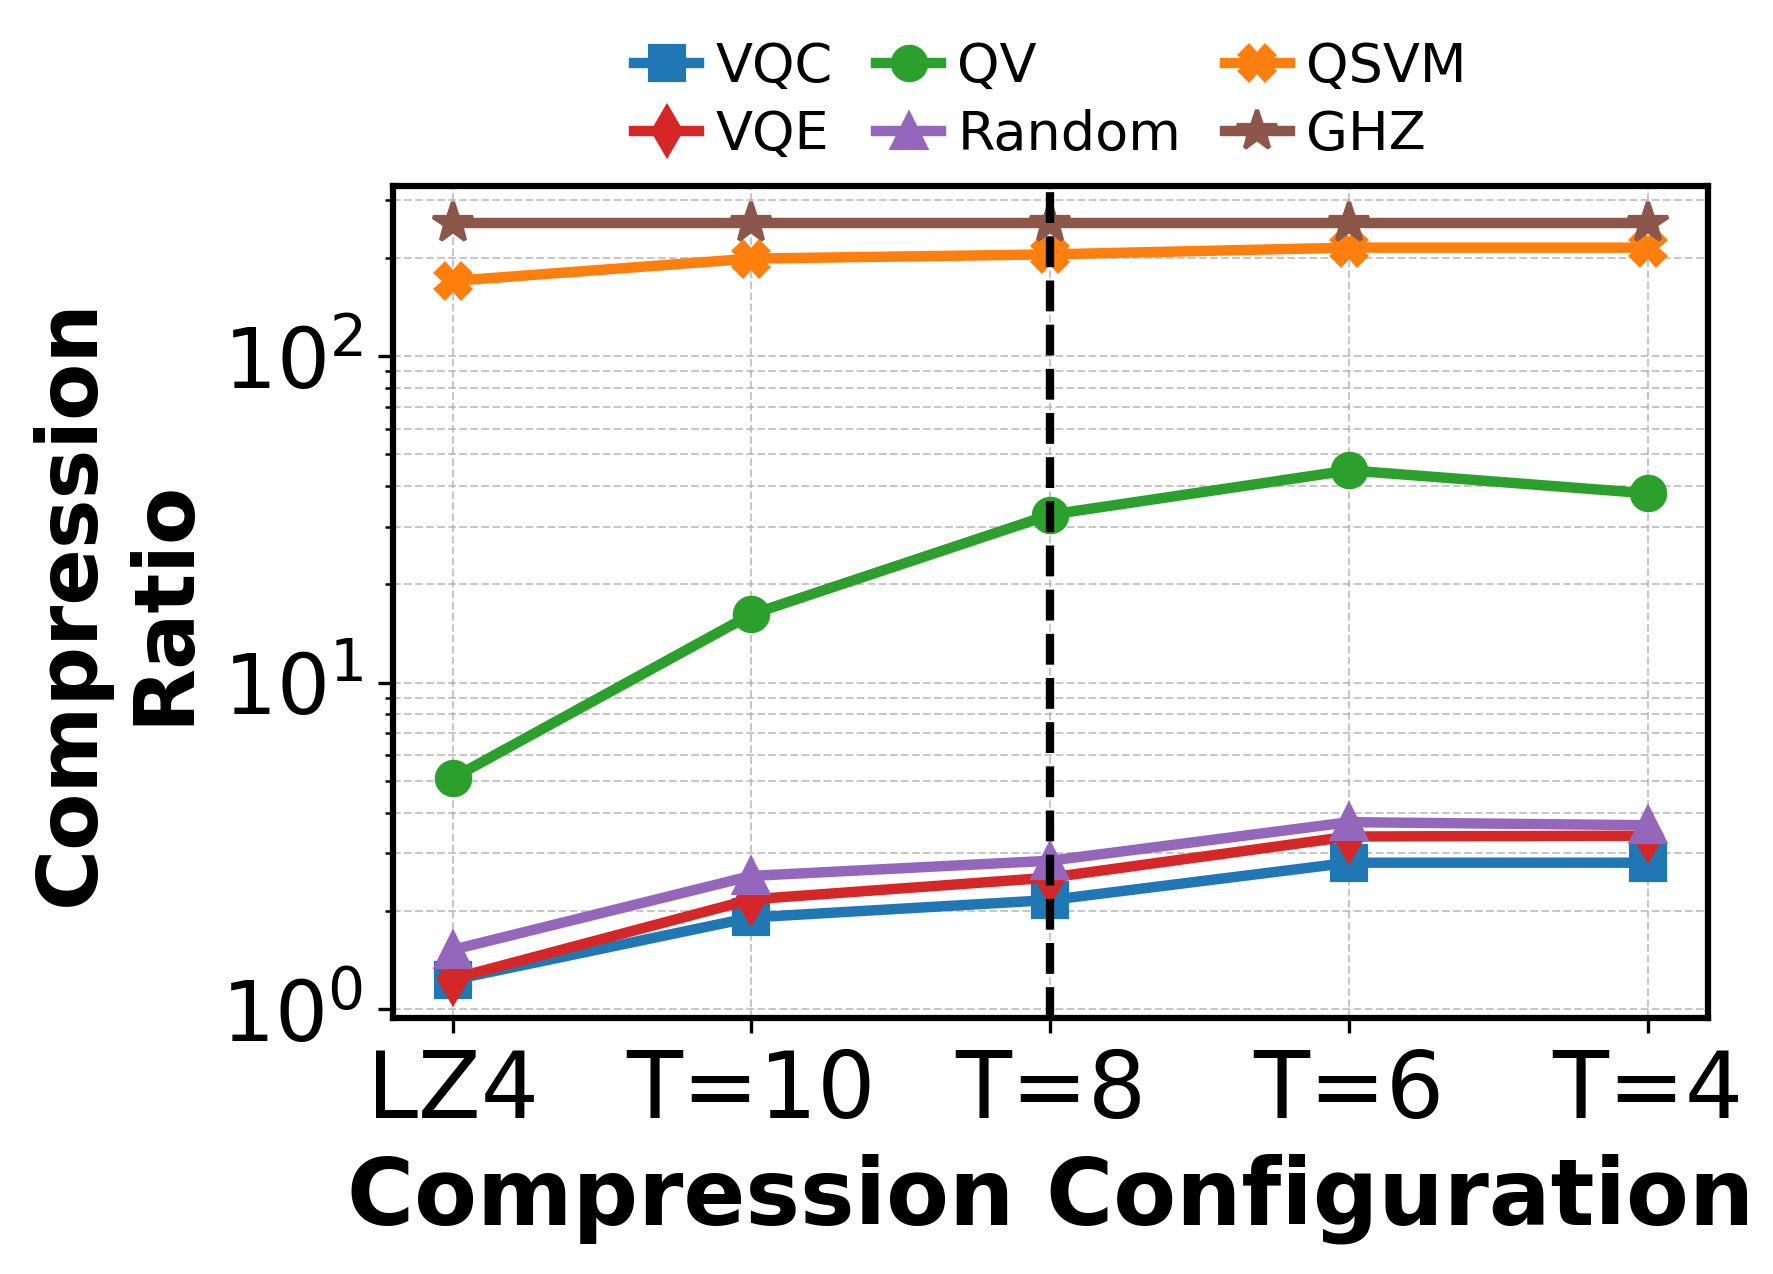
\includegraphics[width=\linewidth]{Figures/compress1.png}
        \caption{Compression ratio across truncation depths.}
        \label{fig:eff_ratio}
    \end{subfigure}\hfill
    \begin{subfigure}[b]{0.54\columnwidth}
        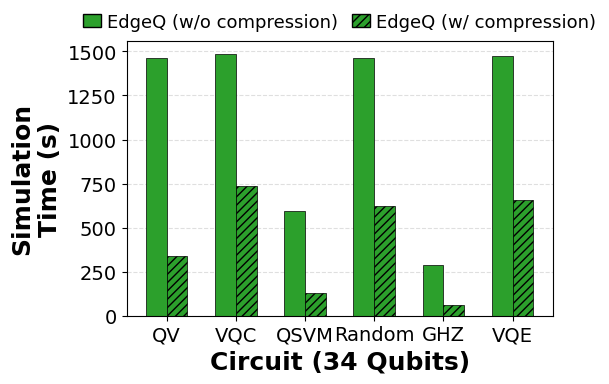
\includegraphics[width=\linewidth]{Figures/compress2.png}
        \caption{Compression speedup at 34 qubits.}
        \label{fig:eff_speedup}
    \end{subfigure}
    \caption{Storage efficiency from mantissa-truncated LZ4 compression.}
    \label{fig:storage_eff}
\end{figure}


Since the 500GB physical NVMe SSD on the Jetson platform cannot accommodate raw state vectors beyond 35 qubits in the dual-file ping-pong layout, \EdgeQuantum uses ping-pong mantissa-truncated LZ4 compression to extend simulation capacity. Figure~\ref{fig:storage_eff} reports two measurements. Figure~\ref{fig:eff_ratio} shows per-circuit compression ratio across the LZ4 baseline and four mantissa truncation depths. Figure~\ref{fig:eff_speedup} shows per-circuit speedup at 34Q, where uncompressed state vectors dominate I/O time.

\noindent\textbf{Compression Ratio Sweep.} Figure~\ref{fig:eff_ratio} compares per-circuit compression ratios across the LZ4 baseline and four mantissa truncation depths. As truncation depth decreases from $T=10$ to $T=8$, the QV ratio expands from 16.2$\times$ to 32.7$\times$, while the VQC ratio scales from 1.91$\times$ to 2.16$\times$. Each truncation depth zeros the lower mantissa bits before LZ4, corresponding to per-file ratios from 2.16$\times$ (VQC) to 255$\times$ (GHZ) at $T=8$ across the six circuits. The byte shuffle groups same-position bytes across amplitudes to expose zero-runs in the truncated lower bytes, yielding ratios above the LZ4-only baseline by up to 6$\times$ for QV. The $T=8$ point reflects the chosen operating depth, whereas $T=6$ further increases the ratio for QV (32.7$\times$$\rightarrow$44.7$\times$) and $T=4$ reduces it (44.7$\times$$\rightarrow$38.0$\times$). Thus, \EdgeQuantum fits a 39-qubit GHZ simulation within 32GB of NVMe storage at $T=8$, whereas dense circuits achieve per-file compression of 2.16$\times$-2.85$\times$ that supports up to 36 qubits within the 500GB capacity.


\noindent\textbf{Performance Benefit.} Figure~\ref{fig:eff_speedup} compares per-circuit simulation time of \EdgeQuantum with and without mantissa-truncated LZ4 compression at 34Q, isolating the compression speedup from capacity necessity since the raw state vector still fits the 500GB SSD without compression. Compression yields a 1.73$\times$-4.59$\times$ speedup across the six circuit types, with the largest gain on GHZ (290.2s $\rightarrow$ 63.3s, 4.59$\times$) and the smallest on VQC (1483.8s $\rightarrow$ 858.2s, 1.73$\times$). This range arises because the per-circuit compression ratio determines I/O reduction between UVM and NVMe, and high-ratio circuits (GHZ, QSVM, QV) transition into a regime dominated by compression and decompression overhead while dense circuits (VQC, Random, VQE) remain partially I/O-bound. At 34Q, all circuits start heavily I/O-bound regardless of compute density, so compression delivers speedup proportional to the I/O reduction it provides. The asynchronous pipeline alone capped GHZ at 1.21$\times$ (Section~\ref{4.2}) because its narrow compute window limited write-latency overlap. Compression bypasses this compute-window dependence by reducing I/O volume directly, so GHZ achieves a 4.59$\times$ speedup that matches the high-ratio circuits (QSVM 4.57$\times$, QV 4.18$\times$) and exceeds the dense circuits (1.73$\times$-2.04$\times$).




\subsection{Extreme Scalability: 35–39 Qubits}


\begin{table}[t]
\centering
\scriptsize
\caption{Extreme-scale simulation times (seconds) for \EdgeQuantum with mantissa-truncated LZ4 compression at $T=8$ (Depth=5). Dash indicates configurations that exceed the 500GB SSD capacity in the dual-file ping-pong layout.}
\resizebox{\columnwidth}{!}{%
\begin{tabular}{|l|r|r|r|r|r|}
\hline
\textbf{Circuit} & \textbf{35Q (256GB)} & \textbf{36Q (512GB)} & \textbf{37Q (1TB)} & \textbf{38Q (2TB)} & \textbf{39Q (4TB)} \\
\hline
GHZ    & 119.10 & 246.77 & 492.53 & 990.21 & 1,980.20 \\
QSVM   & 251.69 & 494.23 & 982.25 & 1,981.10 & 3,974.19 \\
QV     & 650.45 & 1,355.27 & 2,683.68 & 5,445.10 & 10,811.64 \\
\hline
Random & 1,328.69 & 2,739.91 & --- & --- & --- \\
VQE    & 1,486.57 & 2,949.12 & --- & --- & --- \\
VQC    & 1,619.05 & 3,295.61 & --- & --- & --- \\
\hline
\end{tabular}%
}
\label{tab:extreme_results}
\end{table}

Beyond 34 qubits, the logical state vector exceeds the 500GB SSD capacity by up to 8$\times$ (4TB at 39Q). This makes the mantissa-truncated LZ4 ping-pong compression layer mandatory for execution, enabling \EdgeQuantum to operate where alternative simulators fail. Table~\ref{tab:extreme_results} shows the per-circuit simulation times across 35Q (256GB) to 39Q (4TB).

As shown in the table, \EdgeQuantum exhibits stable, near-linear scalability as the state vector doubles at each qubit increment. For high-ratio circuits (GHZ, QSVM, QV), runtime tracks the 16$\times$ data volume growth, increasing 15.8$\times$$-$16.6$\times$ from 119.1s$-$650.5s at 35Q to 1,980.2s$-$10,811.6s at 39Q (e.g., 10,811.6s or $\approx$3.00 hours for QV). Dense circuits stop at 36Q within the 500GB capacity, with Random, VQE, and VQC completing 36Q in 2,739.9s, 2,949.1s, and 3,295.6s, respectively. This near 2$\times$ time growth per qubit confirms that the ping-pong pipeline maintains compression throughput at the 4~TB scale for high-ratio circuits without degradation from queue contention or fragmentation.

This regime is accessible to \EdgeQuantum because of its UMA-optimized compression path. Server-grade simulators such as \textit{BMQSim} apply compression at the GPU level, relying on VRAM to stage and compress data, which is infeasible on edge devices. When the logical state vector reaches or exceeds the 500GB SSD capacity in the ping-pong layout ($\geq$35Q), the raw state cannot be persisted on disk, leaving \textit{BMQSim-like} with no chunks to stage from storage. Even at smaller scales, dedicating GPU cycles to compression contends with quantum gate kernels for the same compute resources. By performing mantissa-truncated LZ4 compression on the CPU during the I/O offloading phase, \EdgeQuantum exploits otherwise idle CPU cores and preserves GPU compute cycles for quantum gate operations. Among the three baselines defined in Section\ref{setup}, \textit{cuQuantum} variants fail at 29Q because of DRAM exhaustion, and \textit{BMQSim-like} cannot start beyond 34Q because of SSD exhaustion, leaving \EdgeQuantum as the only framework to reach the 4TB regime on this 8GB device.

\subsection{I/O Breakdown with Compression}\label{sec:io_breakdown_compressed}

\begin{table}[t]
\centering
\caption{I/O breakdown (seconds) for \EdgeQuantum with mantissa-truncated LZ4 ping-pong compression across 34-36 qubits.}
\setlength{\tabcolsep}{3pt}
\scriptsize
\resizebox{\columnwidth}{!}{%
\begin{tabular}{|c|c|r|r|r|r|r|r|}
\hline
\textbf{Qubits} & \textbf{Circuit} & \textbf{pread} & \textbf{decomp.} & \textbf{compute} & \textbf{compress} & \textbf{pwrite} & \textbf{Total} \\
\hline
\multirow{3}{*}{34Q}
 & VQC & 158.9 & 226.9 & 12.6 & 84.1 & 375.7 & 858.2 \\
 & GHZ & 0.4 & 44.3 & 2.0 & 15.7 & 0.9 & 63.3 \\
 & VQE & 148.9 & 221.3 & 11.8 & 82.1 & 310.1 & 774.2 \\
\hline
\multirow{3}{*}{35Q}
 & VQC & 348.9 & 421.6 & 25.1 & 157.4 & 666.0 & 1619.0 \\
 & GHZ & 0.5 & 83.3 & 4.1 & 29.6 & 1.6 & 119.1 \\
 & VQE & 275.4 & 426.4 & 24.3 & 159.4 & 601.0 & 1486.5 \\
\hline
\multirow{3}{*}{36Q}
 & VQC & 723.5 & 856.7 & 50.9 & 320.9 & 1343.6 & 3295.6 \\
 & GHZ & 1.0 & 172.8 & 8.0 & 61.8 & 3.2 & 246.8 \\
 & VQE & 578.7 & 847.6 & 49.6 & 314.1 & 1159.1 & 2949.1 \\
\hline
\end{tabular}%
}
\label{tab:io_breakdown_compressed}
\end{table}



Table~\ref{tab:io_breakdown_compressed} decomposes the execution time of \EdgeQuantum with mantissa-truncated LZ4 ping-pong compression into physical I/O, CPU compression, and GPU compute phases across 34 to 36 qubits.

\noindent\textbf{Bottleneck Shift for High-Ratio Circuits. }Compression and decompression dominate the total execution time for high-ratio circuits, shifting the primary bottleneck from physical I/O to the CPU. For 34Q GHZ, physical I/O operations (\texttt{pread} and \texttt{pwrite}) account for 1.3s, representing 2.1\% of the 63.3s total execution time. Conversely, CPU-driven LZ4 decompression and compression consume 60.0s, constituting 94.8\% of the total duration. This profile demonstrates that the 255$\times$ data volume reduction eliminates the NVMe bandwidth constraint. The system transitions into a CPU-bound regime where execution time depends primarily on compression throughput, validating the design trade-off introduced in Section~\ref{design_compression}.

\noindent\textbf{Linear Scaling and Task Overlap. }As the logical state vector scales from 34Q to 36Q, the execution phases exhibit stable linear growth without triggering OS-level thrashing or I/O contention. For GHZ, CPU decompression time scales from 44.3s (34Q) to 172.8s (36Q), approximately doubling per qubit increment. Across all scales, GPU compute time remains a small fraction of total runtime, requiring 2.0s to 50.9s per simulation. Because the combined CPU LZ4 phase exceeds GPU compute by over an order of magnitude, the GPU compute window is fully absorbed by the background offloading tasks. This validates the UMA-optimized compression path, which overlaps CPU LZ4 with GPU gate execution on shared DRAM. By utilizing otherwise-idle CPU cores for LZ4 processing, \EdgeQuantum extends simulation capacity while maintaining predictable scaling across both CPU-bound (high-ratio) and I/O-bound (dense) regimes.



\subsection{Impact of Buffer Depth}
Figure~\ref{fig:buffer_impact} shows the impact of UVM buffer count on simulation performance at two contrasting state vector scales: 32Q (32~GB) and 36Q (512~GB). Other parameters, such as chunk size (256~MB) and circuit depth (5), are fixed to isolate the buffer-depth effect. While a single buffer executes sequentially without overlap, increasing the buffer count to 4 yields the best performance at both scales, achieving 1.04$\times$-1.12$\times$ speedup at 32Q and 1.02$\times$-1.08$\times$ speedup at 36Q across all circuits. This confirms that \EdgeQuantum's asynchronous pipeline hides NVMe write latency by overlapping it with GPU computation, as described in Section~\ref{design_pipeline}. However, increasing the buffer count beyond 4 progressively reduces this benefit, and the degradation amplifies as the state vector grows.

At 32Q, where the working set occupies a moderate fraction of physical memory, 6- and 8-buffer configurations remain marginally faster than the 1-buffer baseline but lose the gain achieved at 4 buffers. At 36Q, where the active working set occupies most of the available DRAM, over-allocation pushes the buffer pool beyond the headroom of physical memory, triggering UVM page faults and OS-level thrashing. As a result, the 8-buffer configuration runs approximately 0.7-0.8\% slower than the 1-buffer baseline for QSVM, Random, and GHZ. Thus, the 4-buffer choice in \EdgeQuantum's \textit{Tiered Mode} (Section~\ref{design_pipeline}) provides the highest pipeline benefit with minimal residency cost and remains stable across the 32Q to 36Q scale-up.


\begin{figure}[!t]
    \centering
    \hspace*{0.09\linewidth}
    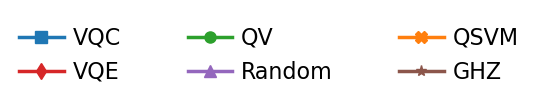
\includegraphics[width=0.6\linewidth]{Figures/lagend_buffers.png}
    \vspace{-.2cm}

    \subfloat[32 Qubits (32\,GB).]{
        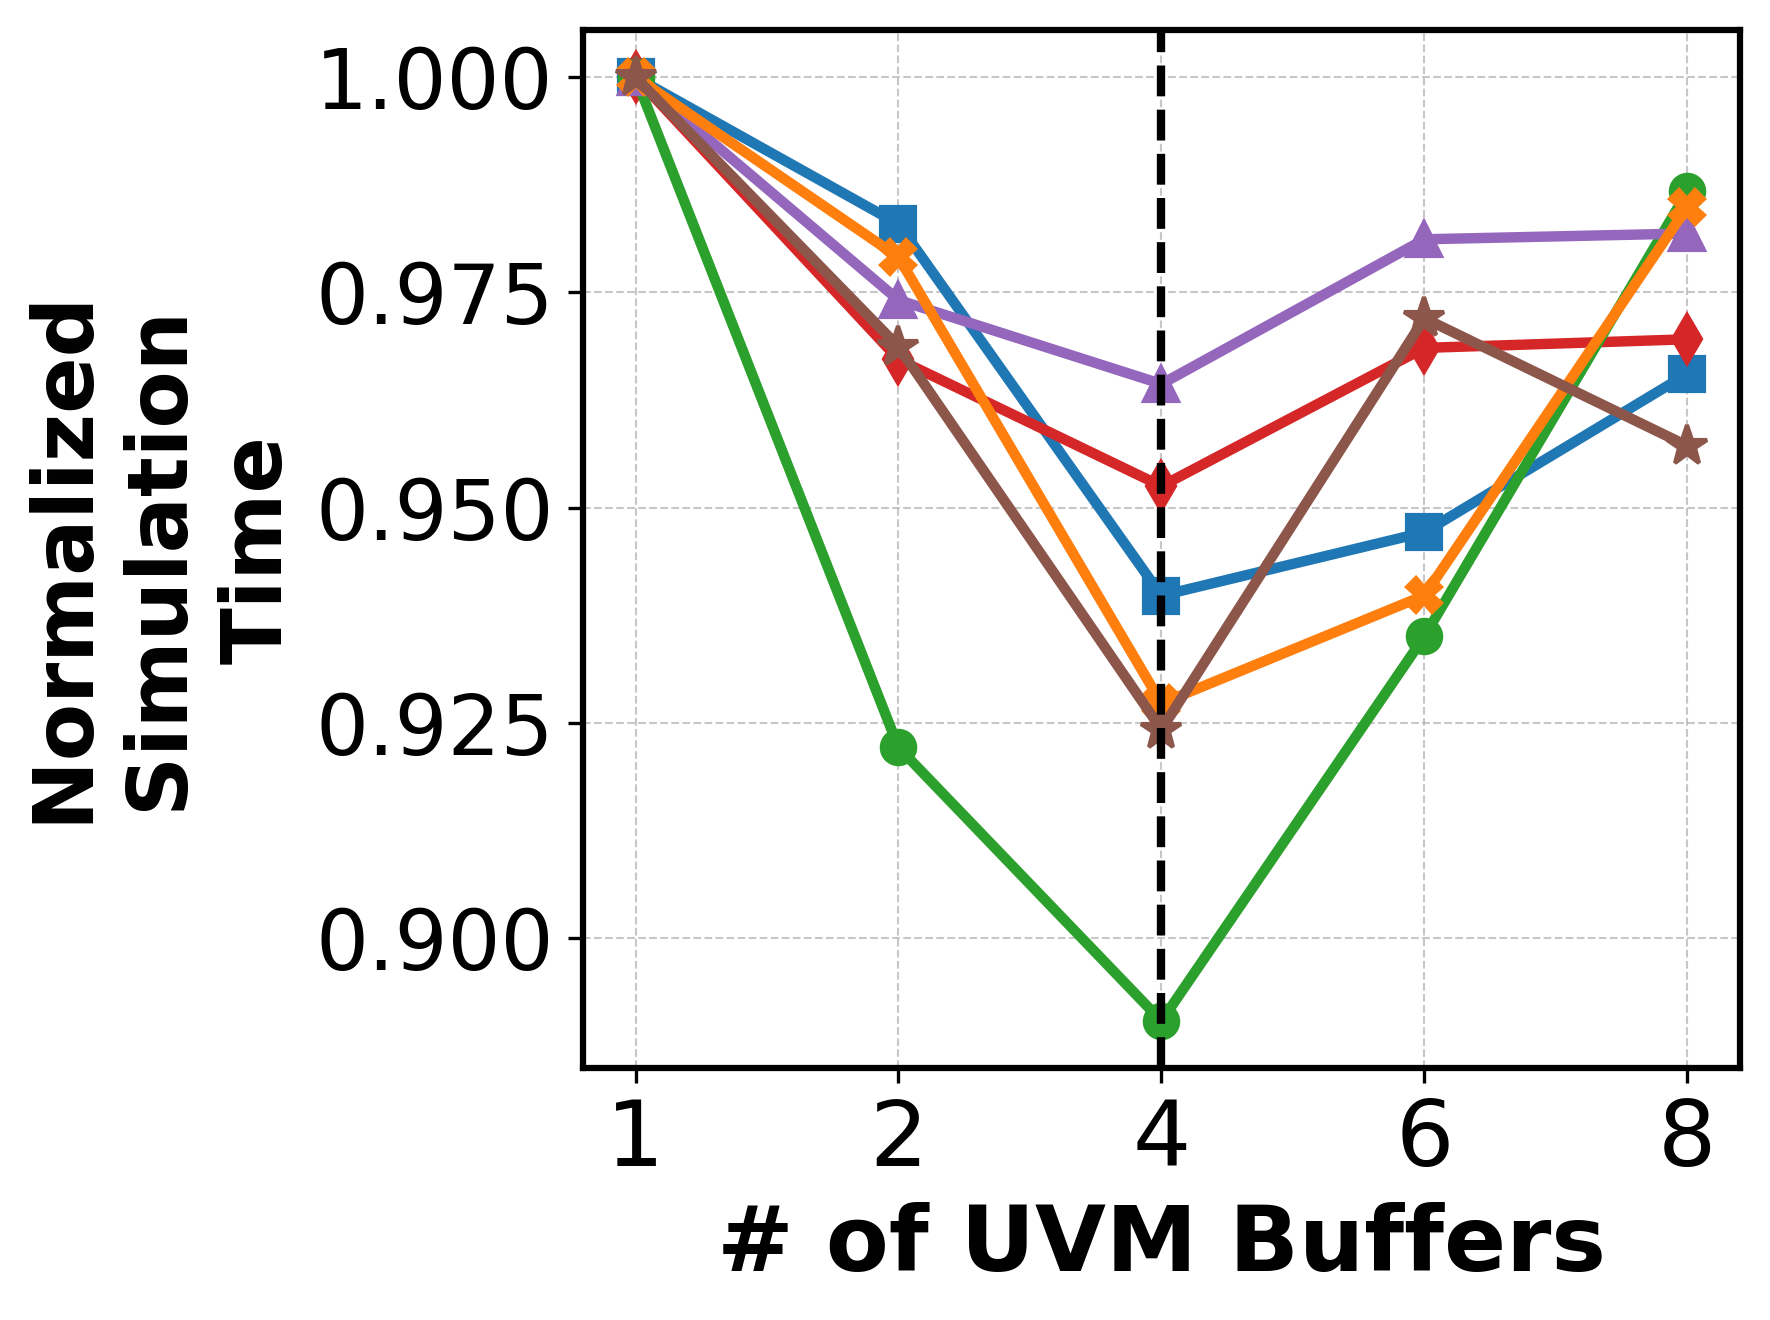
\includegraphics[width=0.46\linewidth]{Figures/32buffer.png}
        \label{fig:buffer_32q}
        \vspace{-.3cm}
    }
    \subfloat[36 Qubits (512\,GB).]{
        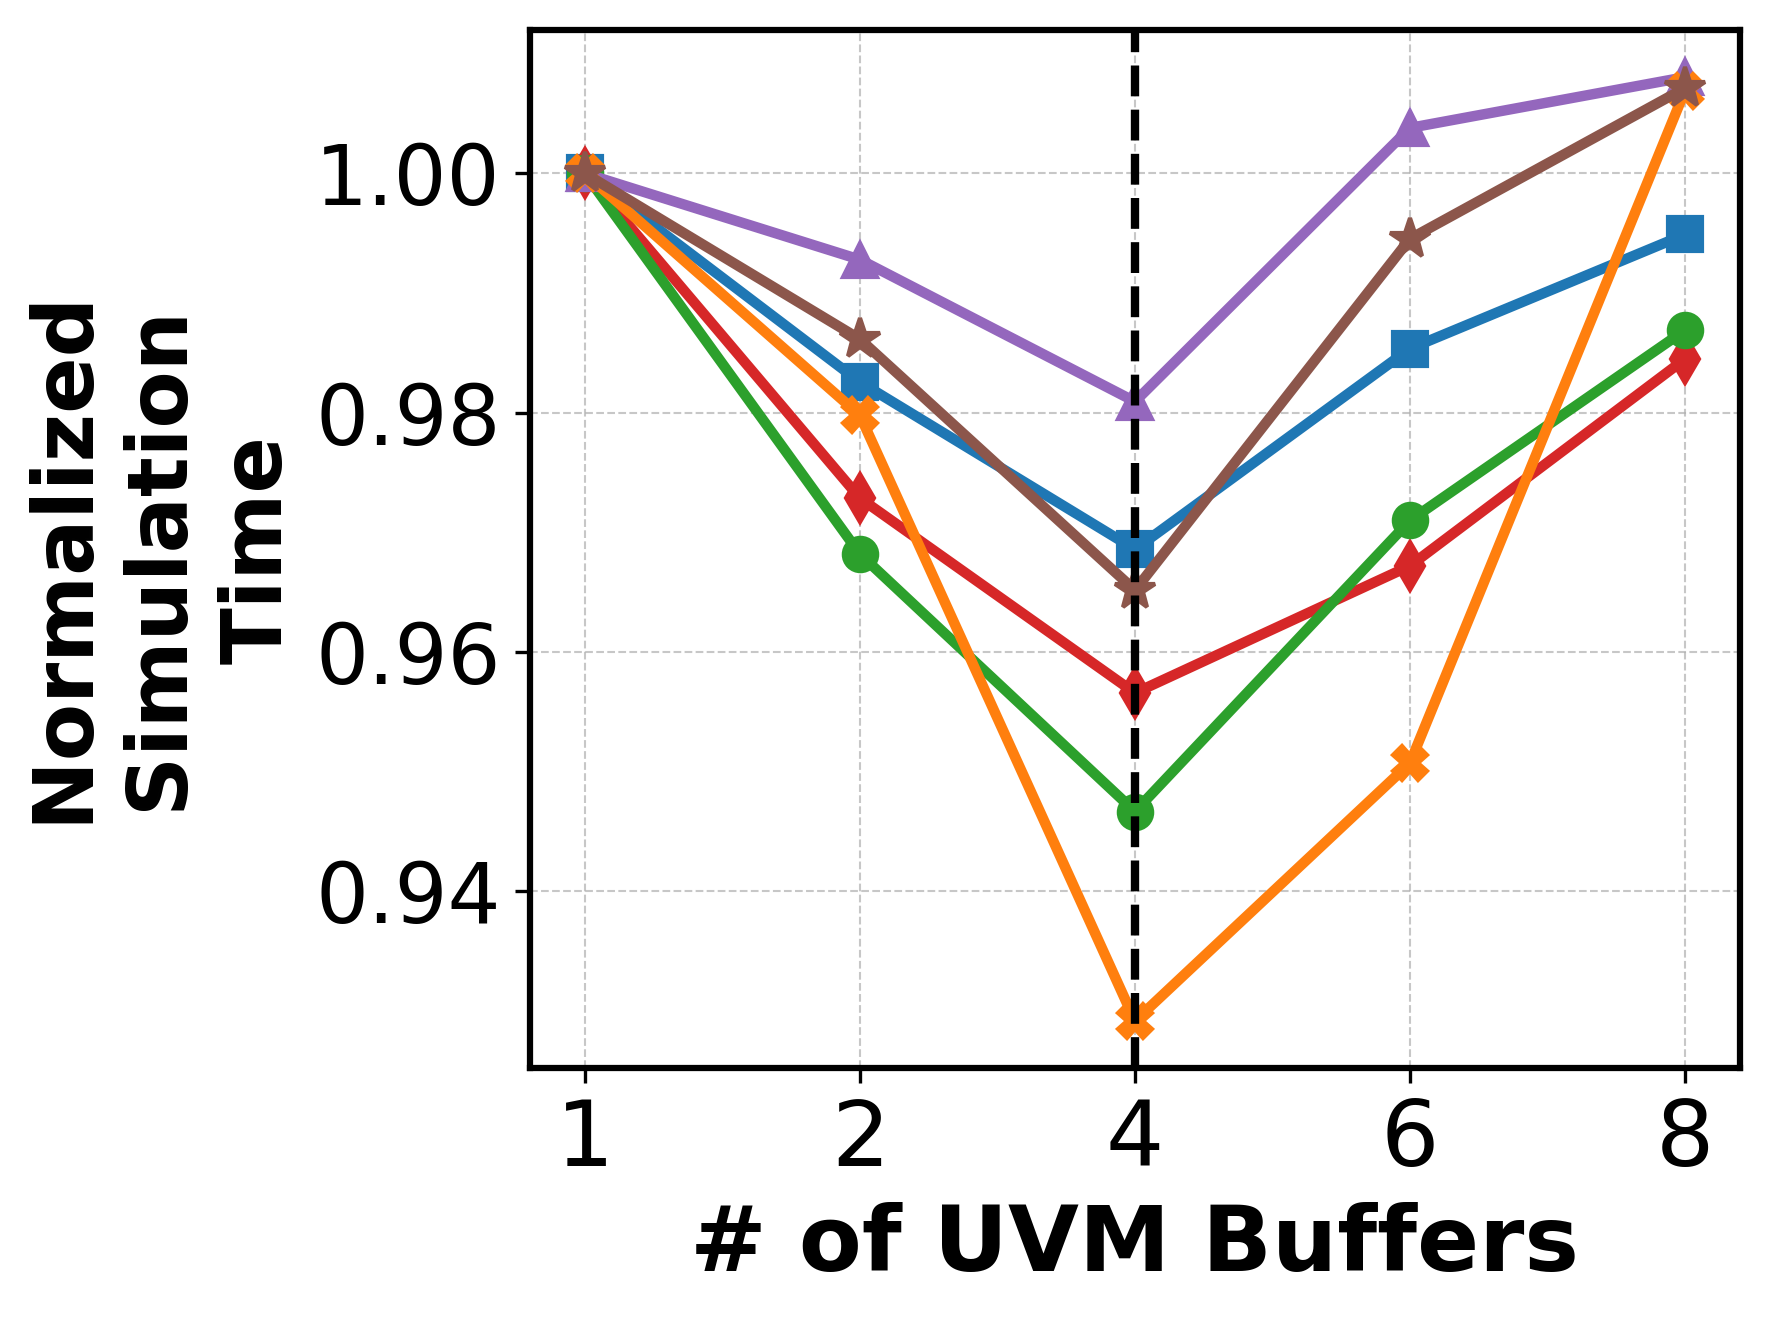
\includegraphics[width=0.46\linewidth]{Figures/36buffer.png}
        \label{fig:buffer_36q}
        \vspace{-.3cm}
    }
    \vspace{-.2cm}
    \caption{Impact of UVM buffer count on simulation time at two state vector scales.}
    \vspace{-.2cm}
    \label{fig:buffer_impact}
\end{figure}


\subsection{Fidelity and Stability}
Since \EdgeQuantum partitions the state vector and relies on frequent I/O, ensuring numerical stability is critical.
We verified the fidelity of the final state vector against small-scale \textit{Cirq} CPU simulations for verifying correctness.

\begin{table}[t]
\centering
\caption{State fidelity $F = |\langle\psi_\text{exact}|\psi_\text{lossy}\rangle|^2$ at depth 5 across truncation depths. Bold column marks the chosen operating depth ($T=8$).}
\label{tab:fidelity}

\setlength{\tabcolsep}{4pt}
\renewcommand{\arraystretch}{1.1}

\footnotesize
\begin{tabular}{c|c|c|c|c}
\hline
\textbf{Circuit} & \textbf{T=10} & \textbf{T=8} & \textbf{T=6} & \textbf{T=4} \\
\hline
GHZ    & 0.9998 & \textbf{0.9998} & 0.9888 & 0.9453 \\
QSVM   & 0.9993 & \textbf{0.9982} & 0.9885 & 0.9553 \\
QV     & 0.9970 & \textbf{0.9919} & 0.9453 & 0.7812 \\
Random & 0.9965 & \textbf{0.9952} & 0.9544 & 0.8213 \\
VQE    & 0.9957 & \textbf{0.9938} & 0.9470 & 0.8114 \\
VQC    & 0.9968 & \textbf{0.9983} & 0.9514 & 0.7900 \\
\hline
\end{tabular}
\end{table}

For all circuits up to 30 qubits (where verification is feasible), Table~\ref{tab:fidelity} reports the measured state fidelity across truncation depths $T \in \{10, 8, 6, 4\}$ at depth 5. At the chosen $T=8$ operating point, fidelity ranges from 0.9919 (QV) to 0.9998 (GHZ), maintaining $F \geq 0.99$ across the six circuits. Lower $T$ values trade fidelity for compression: $T=6$ drops dense circuits to 0.9453--0.9544 and $T=4$ further to 0.78-0.95, while $T=10$ raises all circuits above 0.9957 at the cost of weaker compression (Figure~\ref{fig:eff_ratio}).
The successful completion of 151 benchmark runs without a single crash or I/O error validates the robustness of the 4-buffer pipeline and the UVM management logic.


